\documentclass[letter]{beamer}
%removed: handout (ignores "animations")

\usepackage[utf8]{inputenc}
\usepackage{graphicx}
\usepackage{minted}

\usetheme{AnnArbor}
%\usetheme{CambridgeUS}
\usecolortheme{beaver}

\title[IIC2333] % (optional, only for long titles)
{08 - Capa de Transporte}
\subtitle{IIC2333 - Sistemas Operativos y Redes}
\author[C.Ruz] % (optional, for multiple authors)
{Cristian Ruz -- {\tt cruz@ing.puc.cl}\footnote{Material preparado con aporte del profesor Carlos Buil Aranda} }
\institute[PUC] % (optional)
{
  Departamento de Ciencia de la Computación\\
  Pontificia Universidad Católica de Chile
}
\date[2/2015] % (optional)
{Semestre 2-2015}
\subject{I}

\AtBeginSection[]
{
  \begin{frame}
    \frametitle{Contenidos}
    \tableofcontents[currentsection]
  \end{frame}
}

\begin{document}

%---------------------------------------------------------------------
\frame{\titlepage}


%---------------------------------------------------------------------
\begin{frame}
\frametitle{Contenidos}
%\tableofcontents[currentsection]
\tableofcontents
\end{frame}


%---------------------------------------------------------------------
\section{Elementos de Transporte}

\begin{frame}
  \frametitle{Capa de Transporte}

  Objetivo: Establecer comunicación entre dos procesos
  
  ¿Y las demás capas qué?
  
  \begin{itemize}
    \item Capa de Enlace: comunicación a través de un enlace
    \item Capa de Red: enrutamiento de {\em host} a {\em host}
    \item Capa de Transporte: comunicación {\bf lógica} entre {\em hosts}
  \end{itemize}  

  Relación con otras capas  
  \begin{itemize}
    \item Servicio usado por la capa de aplicación
    \item Utiliza servicios de la capa de red
  \end{itemize}
\end{frame}

%---------------------------------------------------------------------
\begin{frame}
  \frametitle{Capa de Transporte}
  
  Protocolos de transporte transmiten información de un proceso en {\em host} emisor a un proceso en {\em host} receptor
  \begin{itemize}
    \item {\bf Emisor}: recibe un mensaje de capa de aplicación, lo divide en segmentos,
          y solicita a la capa de red que envíe los segmentos al receptor
    \item {\bf Receptor}: recibe segmentos, los ensambla para formar el mensaje, y lo entrega a la capa de aplicación
  \end{itemize}
  
  Dos protocolos representativos de medios de transporte
  \begin{itemize}
    \item TCP
    \item UDP
  \end{itemize}
\end{frame}

%---------------------------------------------------------------------
\begin{frame}
  \frametitle{Protocolos de Transporte}
  \framesubtitle{¿Cómo quiere su entrega?}
  
  Entrega confiable y ordenada (TCP)
  \begin{itemize}
    \item Control de congestión, control de flujo, y establecimiento de conexión
  \end{itemize}
  Entrega no confiable y desordenada (UDP)
  \begin{itemize}
    \item Mejor esfuerzo posible
  \end{itemize}


  \begin{center}
    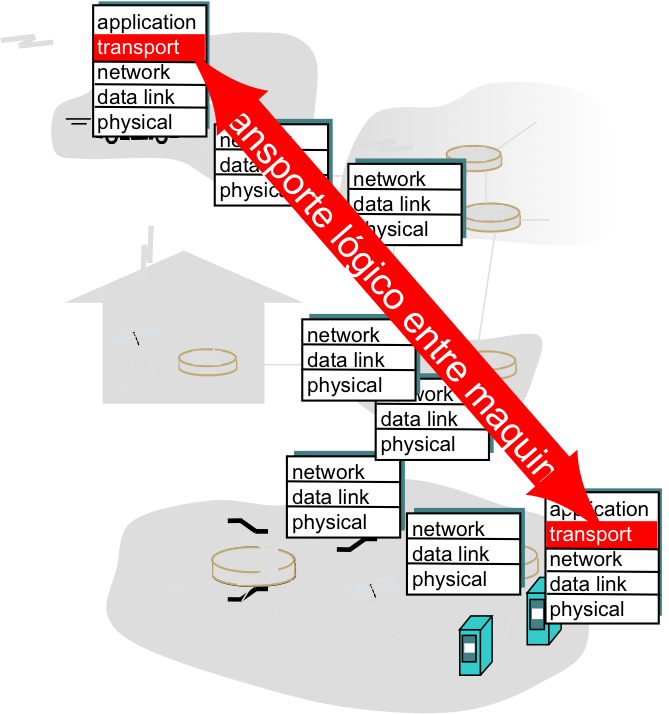
\includegraphics[width=5cm]{figs/08-transporte.png}
  \end{center}

\end{frame}

%---------------------------------------------------------------------
\begin{frame}
  \frametitle{Formato de Segmento}

  Mensaje es dividido en segmentos
  \begin{itemize}
    \item Segmentos se transmiten en paquetes IP
  \end{itemize}
  ¿Cómo identificar mensajes a distintos procesos?
  \begin{itemize}
    \item Se utiliza un {\bf puerto} para establecer diferencias
          entre procesos de origen y destino dentro de un mismo emisor o receptor
    \item Multiplexación de mensajes
  \end{itemize}

  \begin{center}
    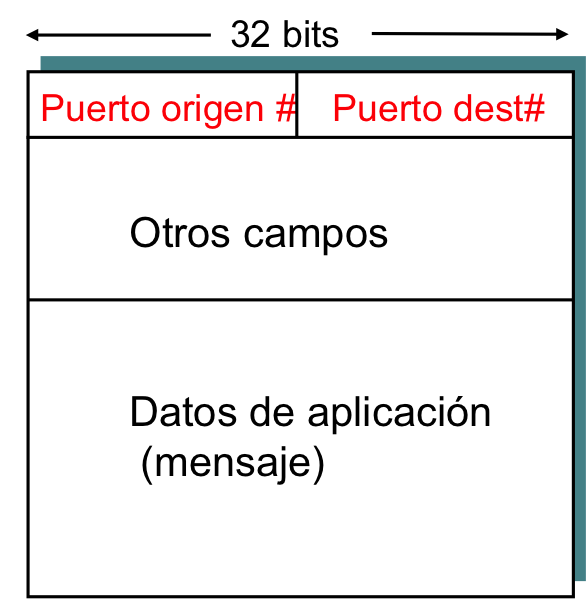
\includegraphics[width=4cm]{figs/08-segmento.png}
  \end{center}

\end{frame}
%---------------------------------------------------------------------
\begin{frame}
  \frametitle{Demultiplexación sin conexión}

  Cada aplicación (proceso) crea mensajes con número de puerto de específico
  \begin{itemize}
    \item Segmento UDP: $\langle$IP destino, puerto destino$\rangle$
  \end{itemize}
  {\em Host} receptor
  \begin{itemize}
    \item Observa el puerto de destino
    \item Pasa el segmento al proceso asociado al puerto de destino
  \end{itemize}

\end{frame}

%---------------------------------------------------------------------
\begin{frame}
  \frametitle{Demultiplexación orientada a la conexión}

  Segmento TCP se identifica con 4 elementos:
  \begin{itemize}
    \item IP origen, puerto origen
    \item IP destino, puerto destino
  \end{itemize}
  Servidores pueden gestionar múltiples conexiones TCP
  \begin{itemize}
    \item Se pueden asociar distintos sockets a distintos clientes
  \end{itemize}
\end{frame}
%---------------------------------------------------------------------
%\section{Control de Congestión}

%---------------------------------------------------------------------
\section{UDP}

\begin{frame}
  \frametitle{UDP: User Datagram Protocol}
  
  \begin{itemize}
    \item Servicio de ``mejor esfuerzo'' (best-effort)
    \item Segmentos pueden perderse
    \item Segmentos pueden llegar y entregarse a capa de aplicación en distinto orden
  \end{itemize}
  Servicio {\bf no orientado a conexión} ({\em connection-less})
  \begin{itemize}
    \item No se establece conexión previa
    \item Cada segmento UDP se gestiona de manera independiente
  \end{itemize}
\end{frame}

%---------------------------------------------------------------------
\begin{frame}
  \frametitle{UDP: User Datagram Protocol}

  Si entrega tan pocas garantías \ldots ¿para qué?
  \begin{itemize}
    \item Envío simple. Poco {\em overhead} en emisor y receptor.
    \item Procesamiento más rápido
    \item Encabezados más livianos
    \item Si la red es confiable habrá pocas pérdidas
    \item Sin gestión de congestión: se puede enviar a cualquier velocidad
  \end{itemize}

\end{frame}
%---------------------------------------------------------------------
\begin{frame}
  \frametitle{UDP: User Datagram Protocol}

  \begin{itemize}
    \item Frecuente en servicios multimedia
      \begin{itemize}
        \item Servicios multimedia pueden tolerar pérdidas
        \item Tasa de transferencia es más importante que integridad
      \end{itemize}
    \item Usado también en DNS, SNMP
    \item ¿Y si se quiere agregar confiabilidad sin sacrificar tasa de transporte?
      \begin{itemize}
        \item Se pueden agregar chequeos en capa de aplicación
      \end{itemize}
  \end{itemize}

  \begin{center}
    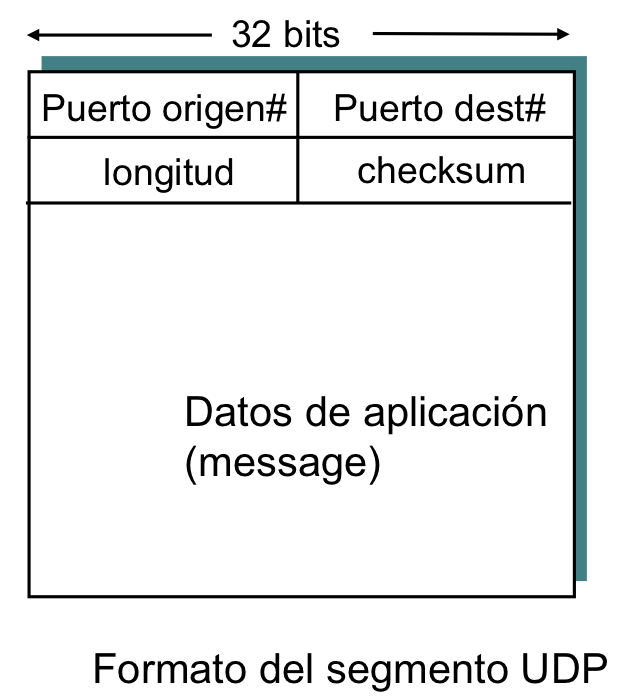
\includegraphics[width=5cm]{figs/08-segmento-udp.png}
  \end{center}


\end{frame}

%---------------------------------------------------------------------
\section{TCP}

\begin{frame}
  \frametitle{Transferencia fiable (Reliable Data Transfer)}
  
  La situación:  
  \begin{itemize}
    \item Diseñar un protocolo que permita comunicación fiable
      \begin{itemize}
        \item Todos los paquetes deben ser recibidos
        \item Saber si algún paquete no ha podido ser entregado
      \end{itemize}
    \item Desafío: debe funcionar sobre un enlace no-fiable (IP)
  \end{itemize}

  \begin{center}
    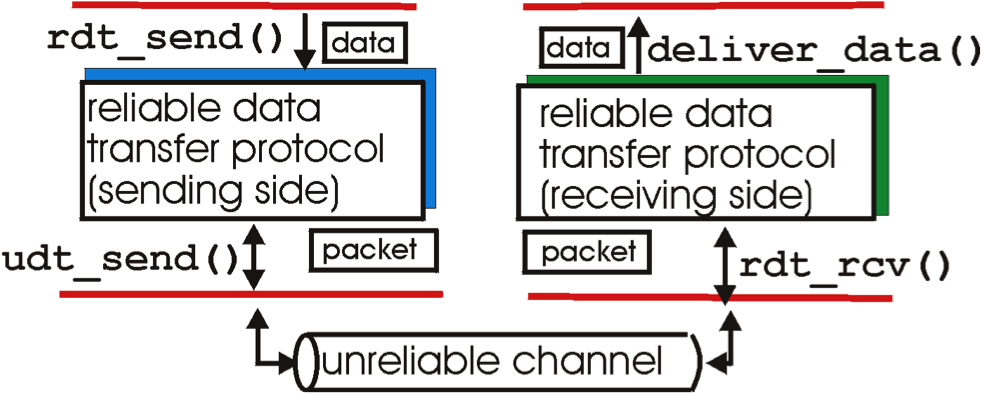
\includegraphics[width=7cm]{figs/08-rdt-1.png}
  \end{center}

\end{frame}

%---------------------------------------------------------------------
\begin{frame}
  \frametitle{{\em Reliable Data Transfer}}

  Caso simple: canal confiable
  \begin{itemize}
    \item Canal de transmisión no pierde paquetes
    \item No se requieren bits de error
  \end{itemize}
  Se modela como una máquina de estados
  
  \begin{center}
    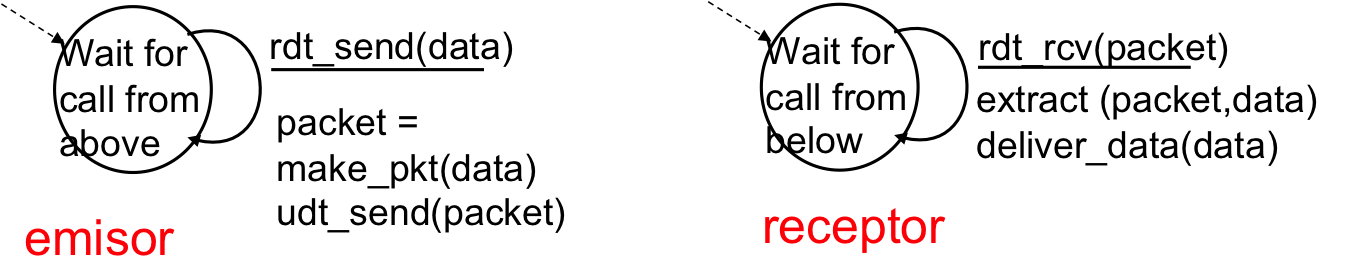
\includegraphics[width=8cm]{figs/08-rdt-2.png}
  \end{center}

\end{frame}
%---------------------------------------------------------------------
\begin{frame}
  \frametitle{{\em Reliable Data Transfer}}

  Canal reales puede modificar los bits
  \begin{itemize}
    \item Mensajes {\bf ACK}: receptor responde explícitamente indicando que el paquete fue recibido
    \item Mensajes {\bf NACK}: receptor responde explícitamente indicando que el paquete contenía errores
    \item Al recibir un {\bf NACK}, el emisor reenvía el paquete
  \end{itemize}
  Dos características nuevas:
  \begin{itemize}
    \item {\em Feedback} del receptor
    \item Mecanismo de retransmisión
  \end{itemize}

\end{frame}

%---------------------------------------------------------------------
\begin{frame}
  \frametitle{{\em Reliable Data Transfer}}

  \begin{center}
    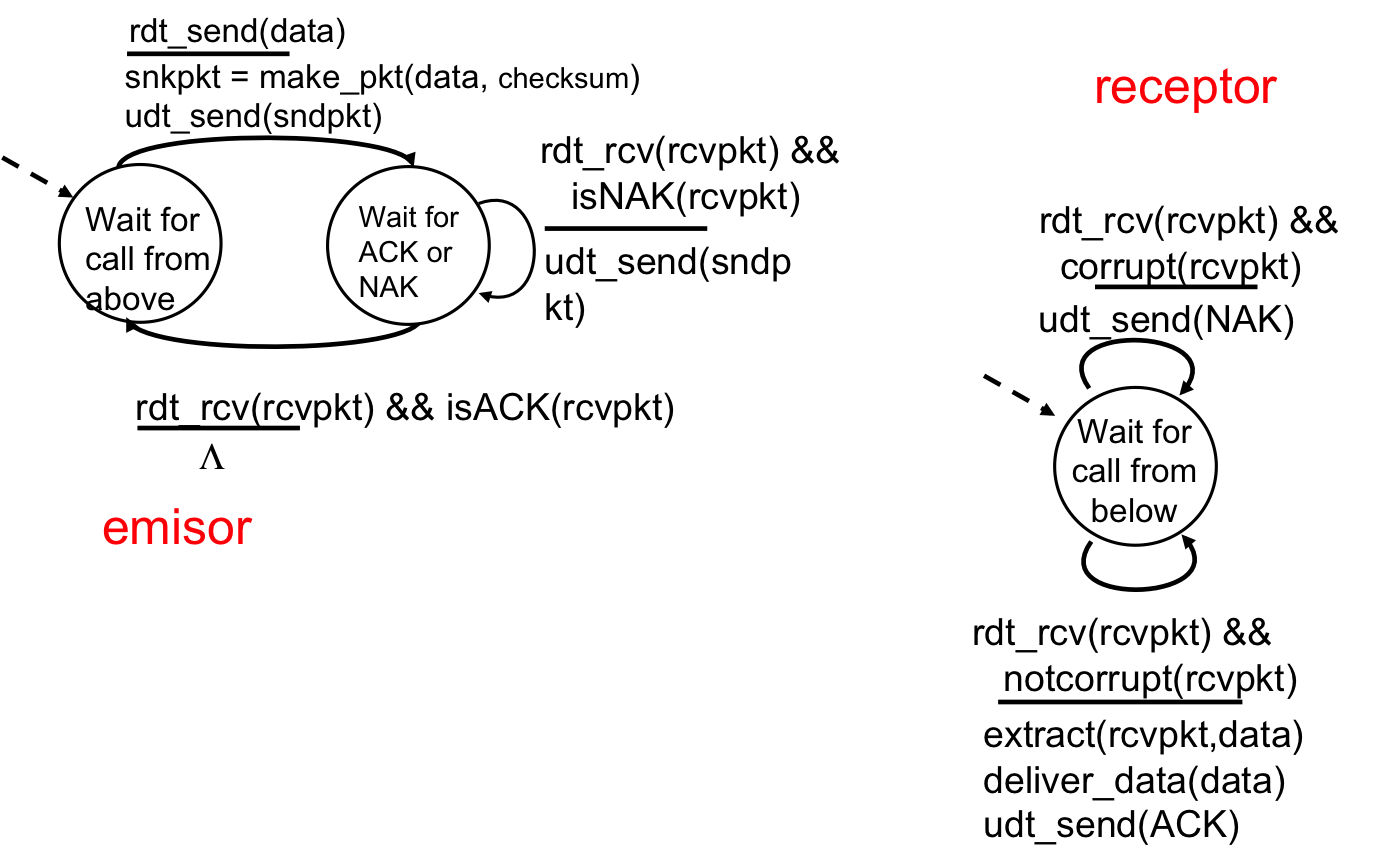
\includegraphics[width=10cm]{figs/08-rdt-3.png}
  \end{center}

\end{frame}

%---------------------------------------------------------------------
\begin{frame}
  \frametitle{{\em Reliable Data Transfer}}

  Problema: ACK o NACK pueden llegar con errores
  \begin{itemize}
    \item Emisor no sabe qué ocurrió en el receptor
  \end{itemize}
  Solución
  \begin{itemize}
    \item Retransmitir si ACK o NACK llegan con errores
    \item Receptor podría recibir duplicados
      \begin{itemize}
        \item Emisor añade número de secuencia a cada paquete
        \item Receptor puede descartar duplicados
        \item Modelo {\bf stop-and-wait}: emisor envía un paquete y espera respuesta
      \end{itemize}
  \end{itemize}

\end{frame}
%---------------------------------------------------------------------
\begin{frame}
  \frametitle{{\em Reliable Data Transfer}}

  Emisor
  \begin{center}
    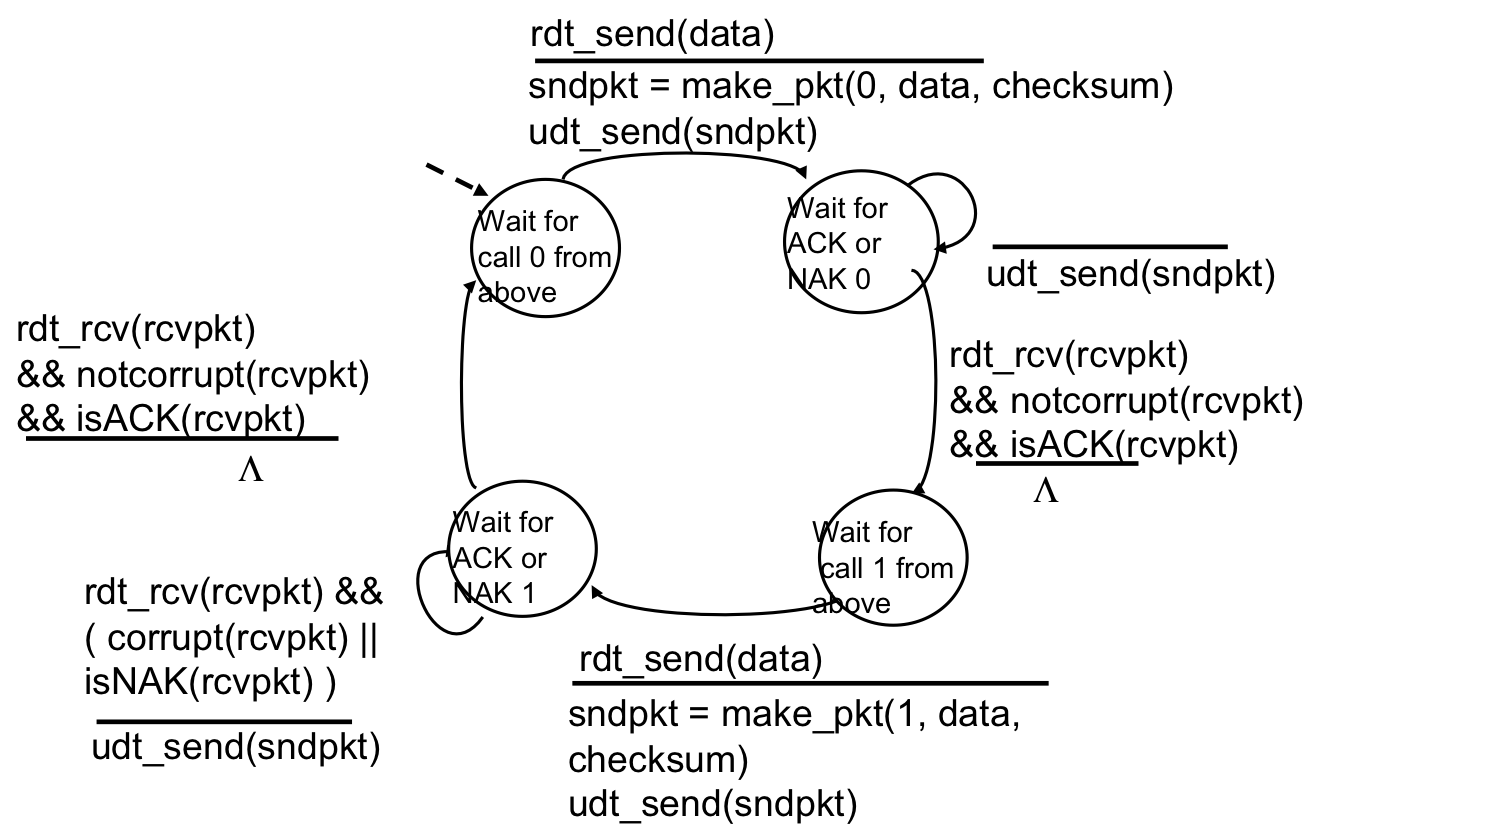
\includegraphics[width=10cm]{figs/08-rdt-4.png}
  \end{center}
  Número de secuencia de 1-bit: 0 ó 1
\end{frame}
%---------------------------------------------------------------------
\begin{frame}
  \frametitle{{\em Reliable Data Transfer}}

  Receptor
  \begin{center}
    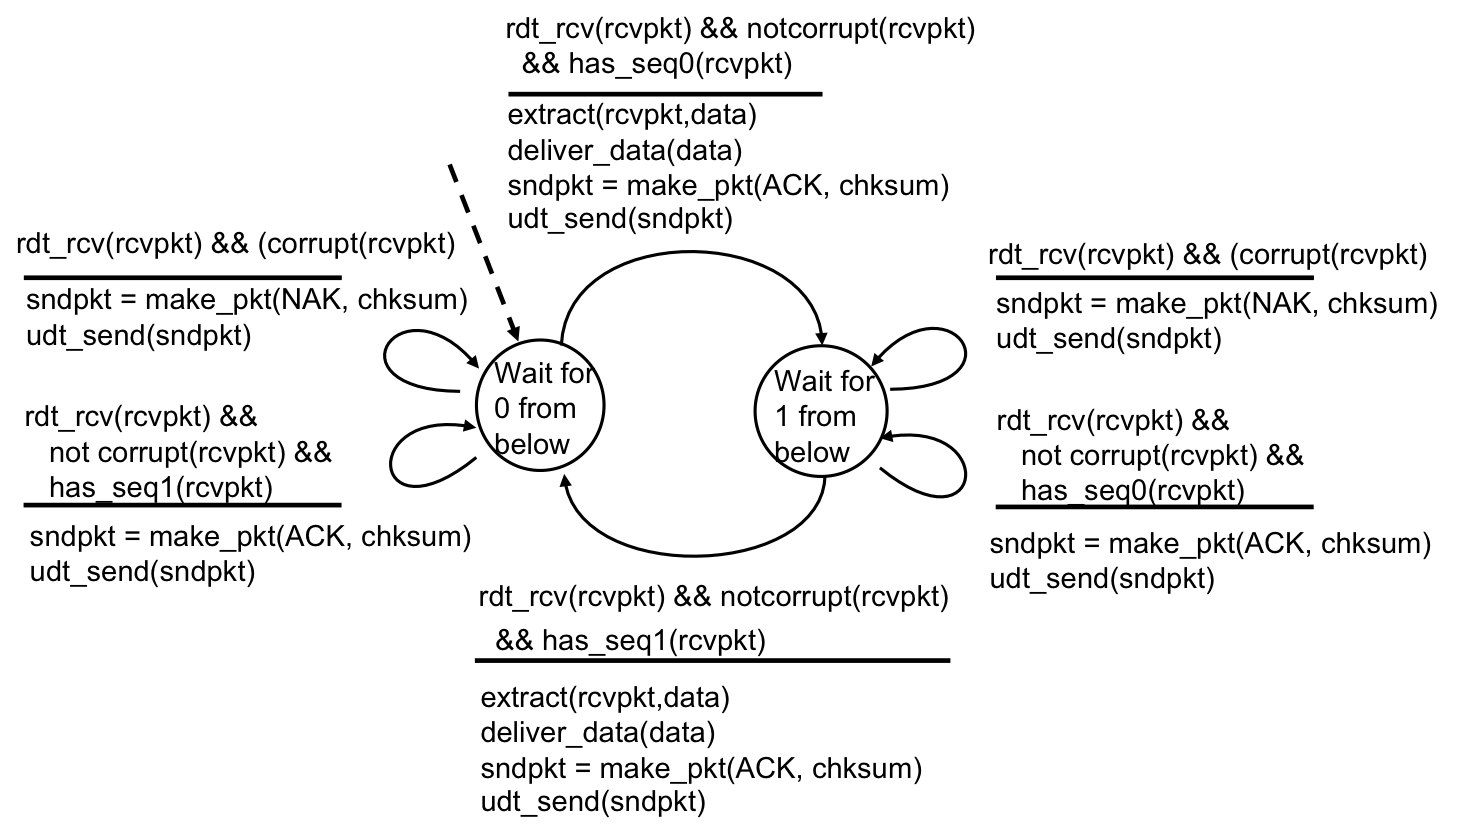
\includegraphics[width=10cm]{figs/08-rdt-5.png}
  \end{center}

\end{frame}

%---------------------------------------------------------------------
\begin{frame}
  \frametitle{{\em Reliable Data Transfer}}

  Problema: paquete no sólo pueden llegar con errores; también pueden perderse
  \begin{itemize}
    \item ACKs, NACKs pueden perderse
    \item Receptor no sabe qué pasó con su último ACN/NACK
  \end{itemize}
  Solución: temporizador
  \begin{itemize}
    \item Emisor espera durante un tiempo determinado los ACK
    \item Si no se reciben ACKs, se retransmite
      \begin{itemize}
        \item Números de secuencia permiten manejar duplicados
        \item Receptor debe indicar numero de secuencia asociado al ACK, NACK
      \end{itemize}
  \end{itemize}

\end{frame}
%---------------------------------------------------------------------
\begin{frame}
  \frametitle{{\em Reliable Data Transfer}}

  Emisor
  \begin{center}
    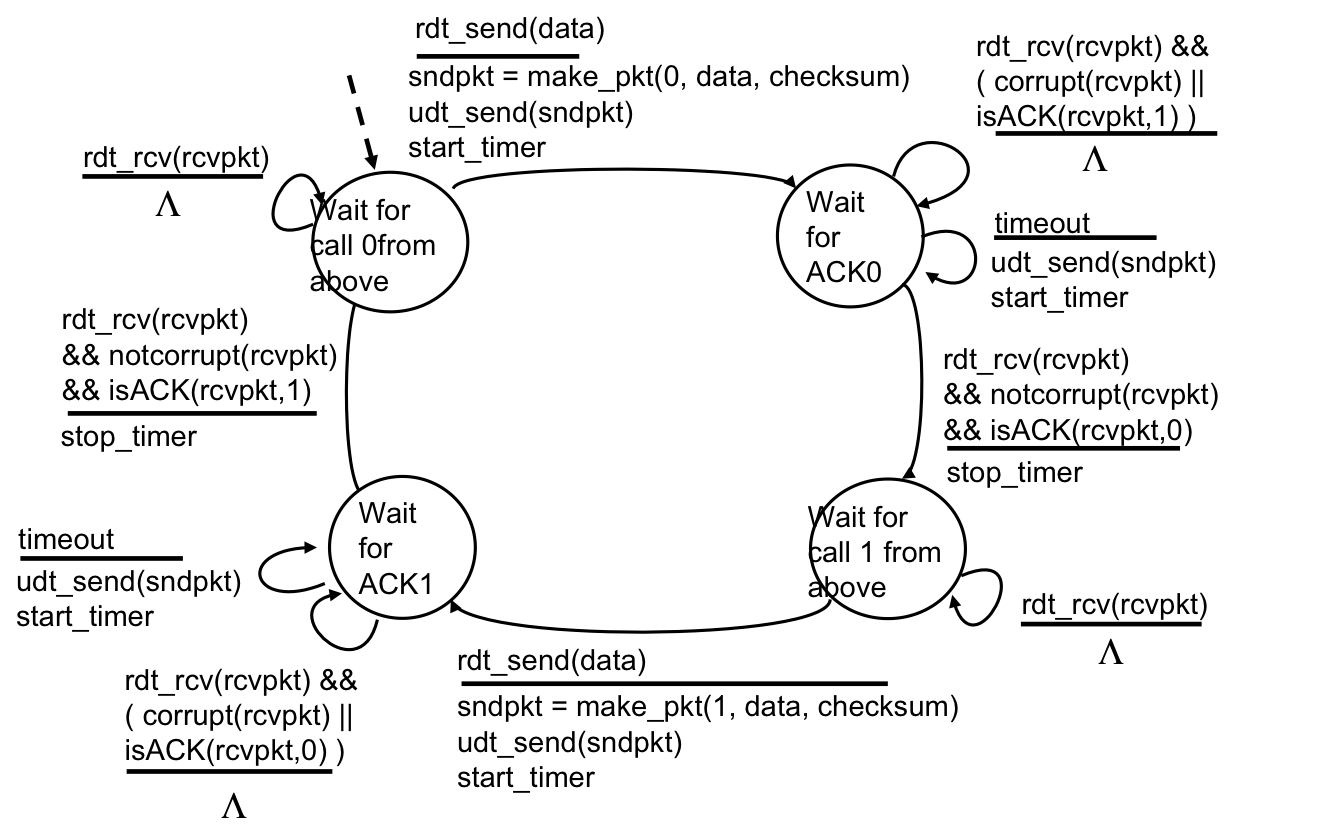
\includegraphics[width=10cm]{figs/08-rdt-6.png}
  \end{center}

\end{frame}

%---------------------------------------------------------------------
\begin{frame}
  \frametitle{{\em Reliable Data Transfer}}

  \begin{center}
    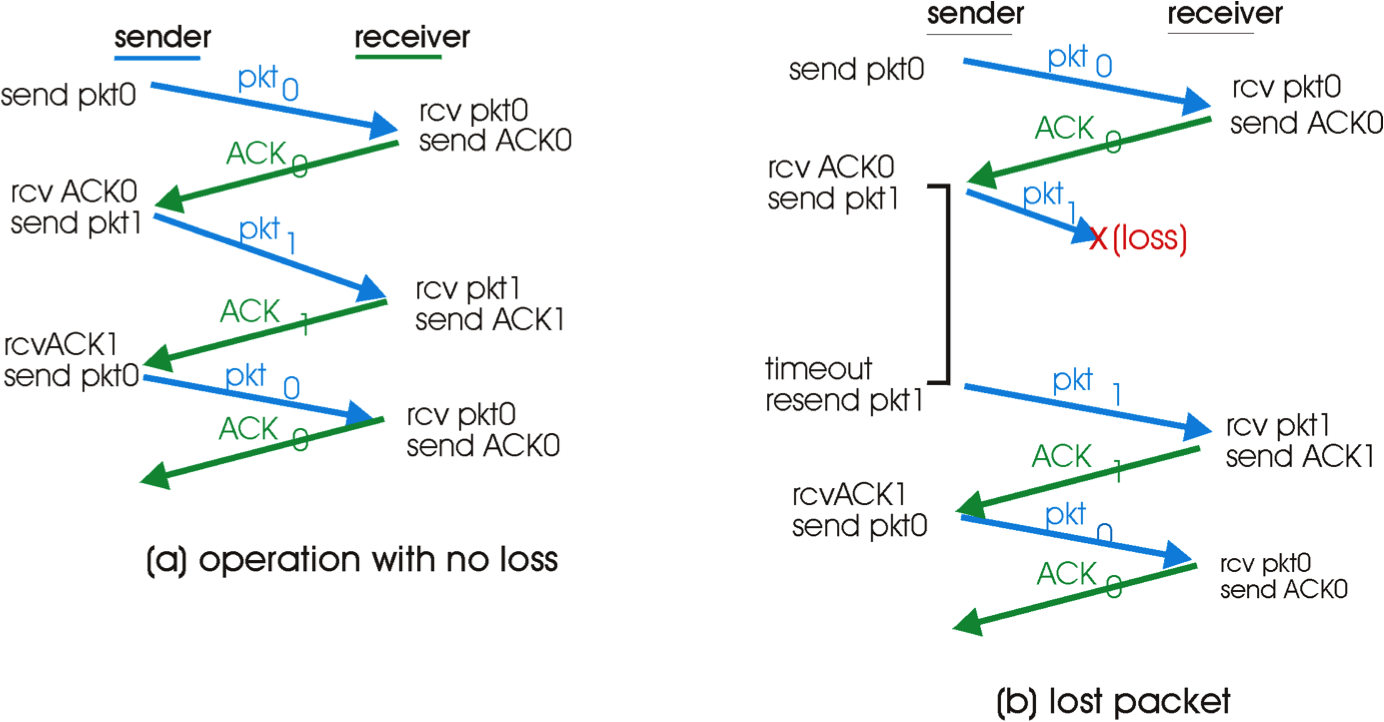
\includegraphics[width=10cm]{figs/08-rdt-7.png}
  \end{center}


\end{frame}
%---------------------------------------------------------------------
\begin{frame}
  \frametitle{{\em Reliable Data Transfer}}

  \begin{center}
    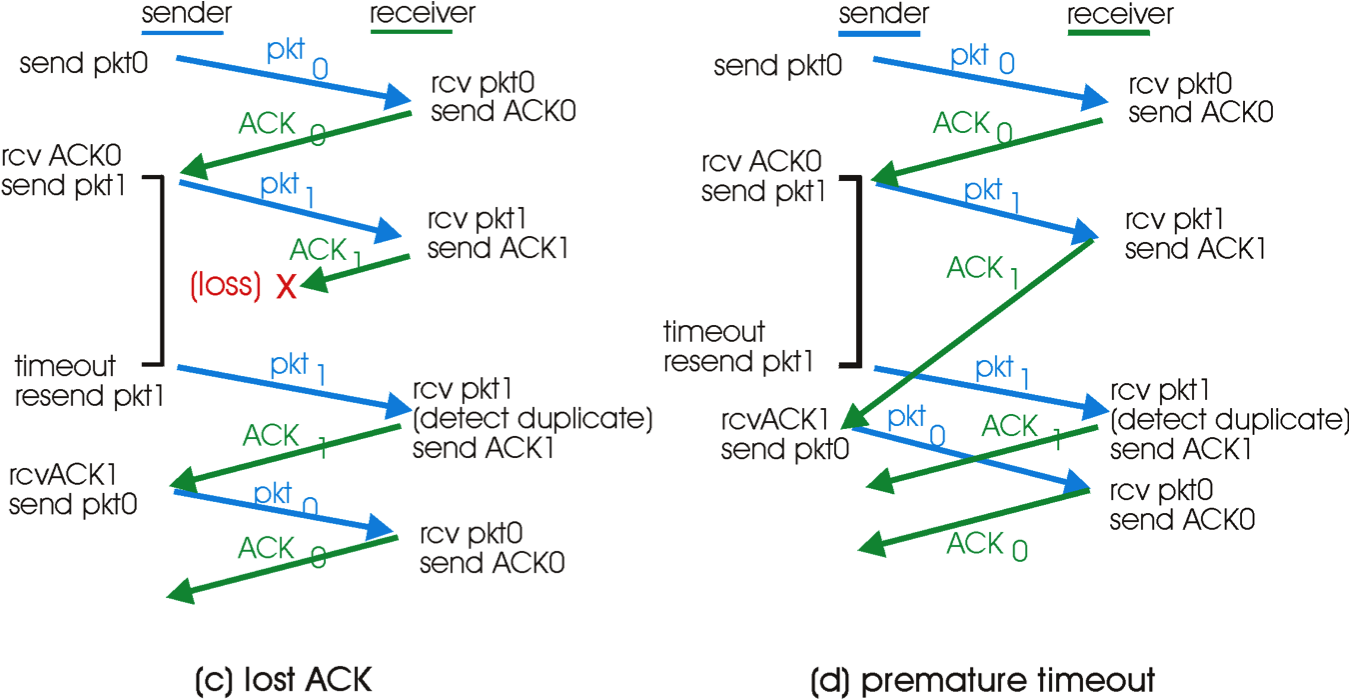
\includegraphics[width=10cm]{figs/08-rdt-8.png}
  \end{center}


\end{frame}

%---------------------------------------------------------------------
\begin{frame}
  \frametitle{{\em Reliable Data Transfer}}

  Utilización del emisor
  \begin{center}
    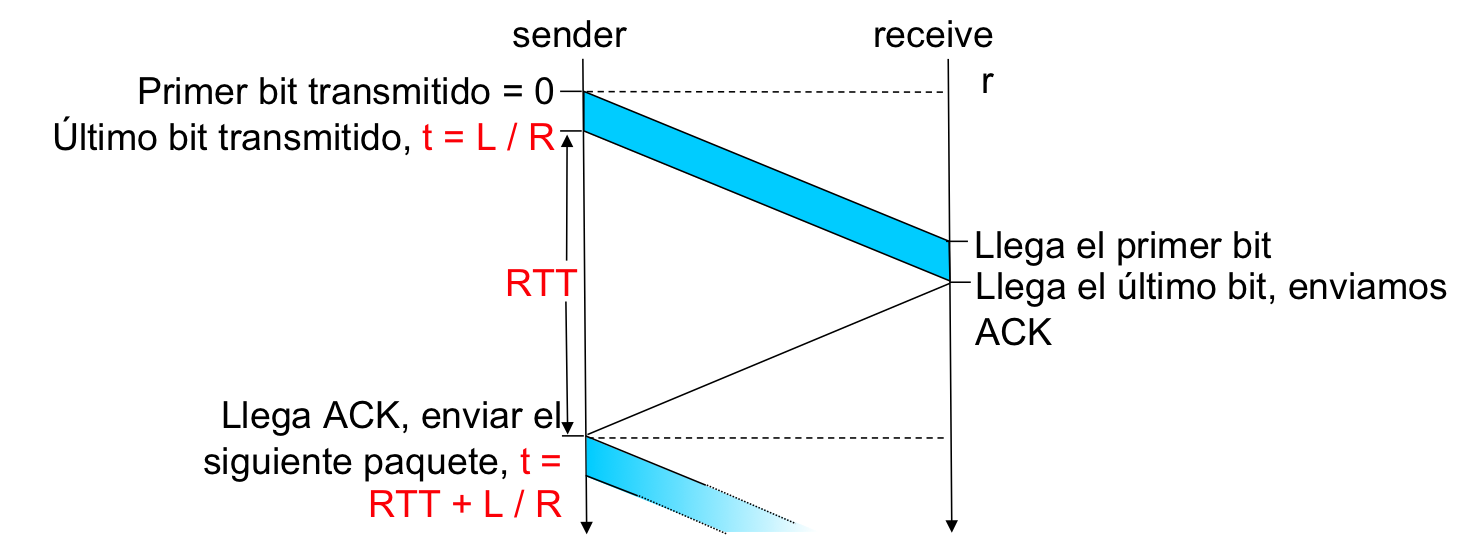
\includegraphics[width=11cm]{figs/08-rdt-9.png}
  \end{center}

\end{frame}
%---------------------------------------------------------------------
\begin{frame}
  \frametitle{{\em Reliable Data Transfer}}

  Enlace de 1Gpbs. Paquetes 8000 bit. 15ms tiempo de transmisión.
  \begin{itemize}
    \item Tiempo para transmitir un paquete:
      \[ \frac{8\times 10^3 \text{bit}}{10^9 \text{bps}} = 8 \times 10^{-6} \text{sec} \]
    \item Round-Trip Time: $2 \times 15 \times 10^{-3} \text{sec} = 30 \times 10^{-3} \text{sec}$
    \item Utilización emisor:
      \[ U_e = \frac{8 \times 10^{-6}}{30\times 10^{-3} + 8\times 10^{-6}} = 0.00027 = 0.027 \% \]
  \end{itemize}

\end{frame}


%---------------------------------------------------------------------
\begin{frame}
  \frametitle{{\em Reliable Data Transfer}}

  Solución: implementaciones ``en cadena'' ({\em chained})
  \begin{itemize}
    \item Envío de múltiples ACK
    \item Rango de número de secuencia incrementales
    \item Requiere buffers en emisor o receptor
    \item Implementaciones:
      \begin{itemize}
        \item Go-Back-N
        \item Repetición Selectiva
      \end{itemize}
  \end{itemize}
\end{frame}

%---------------------------------------------------------------------
\begin{frame}
  \frametitle{{\em Reliable Data Transfer}}

  \begin{center}
    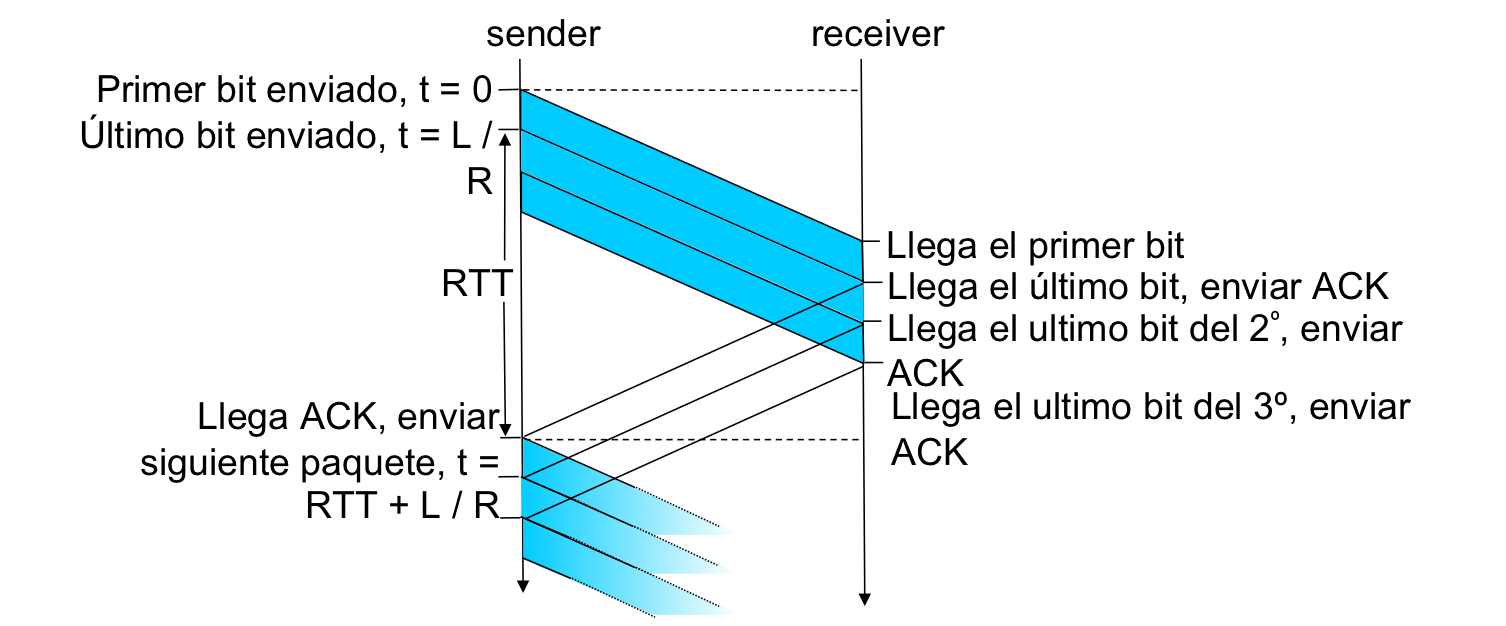
\includegraphics[width=11cm]{figs/08-rdt-10.png}
  \end{center}

\end{frame}
%---------------------------------------------------------------------
\begin{frame}
  \frametitle{{\em Reliable Data Transfer}}

  Enlace de 1Gpbs. Paquetes 8000 bit. 15ms tiempo de transmisión.
  \begin{itemize}
    \item Solo enviando y esperando por grupos de 3 paquetes+ACKs
    \item Tiempo para transmitir un paquete:
      \[ \frac{8\times 10^3 \text{bit}}{10^9 \text{bps}} = 8 \times 10^{-6} \text{sec} \]
    \item Round-Trip Time: $2 \times 15 \times 10^{-3} \text{sec} = 30 \times 10^{-3} \text{sec}$
    \item Utilización emisor:
      \[ U_e = \frac{3\times 8 \times 10^{-6}}{30\times 10^{-3} + 8\times 10^{-6}} = 0.00081 = 0.081 \% \]
  \end{itemize}

\end{frame}
  
%---------------------------------------------------------------------
\begin{frame}
  \frametitle{{\em Reliable Data Transfer}}
  \framesubtitle{Go-Back-N}
  
  \begin{itemize}
    \item Emisor puede mantener hasta $N$ paquetes sin ACK
    \item Receptor envía ACK sólo al recibir correctamente un grupo de paquetes
    \item Emisor usa {\em timer} para paquete más antiguo sin ACK
      \begin{itemize}
        \item Si el {\em timer} expira, se retransmite todo el grupo de paquetes
      \end{itemize}
  \end{itemize}

  \begin{center}
    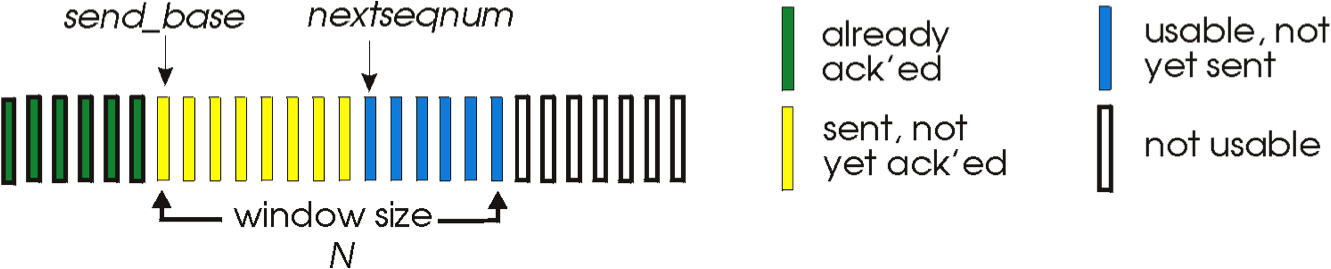
\includegraphics[width=11cm]{figs/08-rdt-11.png}
  \end{center}

\end{frame}
%---------------------------------------------------------------------
\begin{frame}
  \frametitle{{\em Reliable Data Transfer}}
  \framesubtitle{Go-Back-N}

  \begin{center}
    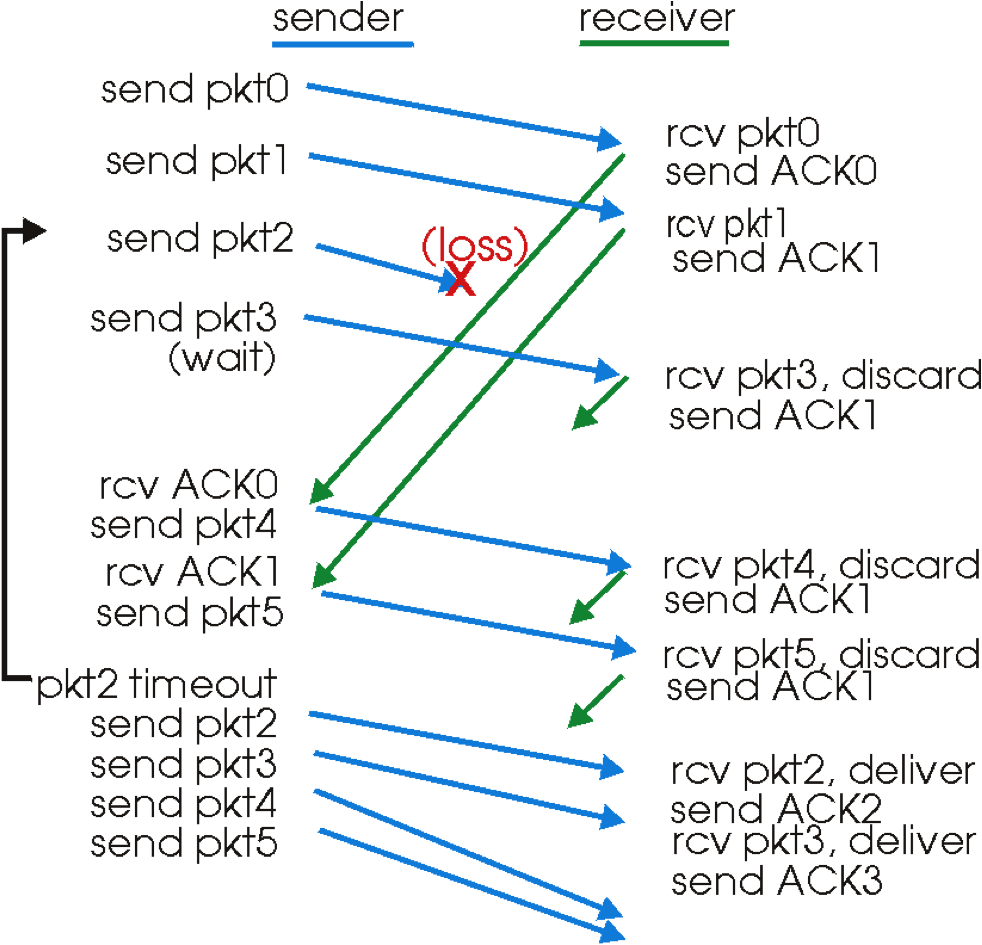
\includegraphics[width=6cm]{figs/08-rdt-12.png}
  \end{center}


\end{frame}
%---------------------------------------------------------------------
\begin{frame}
  \frametitle{{\em Reliable Data Transfer}}
  \framesubtitle{Repetición Selectiva}
  
  \begin{itemize}
    \item Emisor puede mantener hasta $N$ paquetes sin ACK
    \item Receptor envía ACK para cada paquete individual
    \item Emisor usa {\em timer} para paquete más antiguo sin ACK
      \begin{itemize}
        \item Si el {\em timer} expira, se retransmite todo el grupo de paquetes
      \end{itemize}
  \end{itemize}

\end{frame}
%---------------------------------------------------------------------
\begin{frame}
  \frametitle{{\em Reliable Data Transfer}}
  \framesubtitle{Repetición Selectiva}


  \begin{center}
    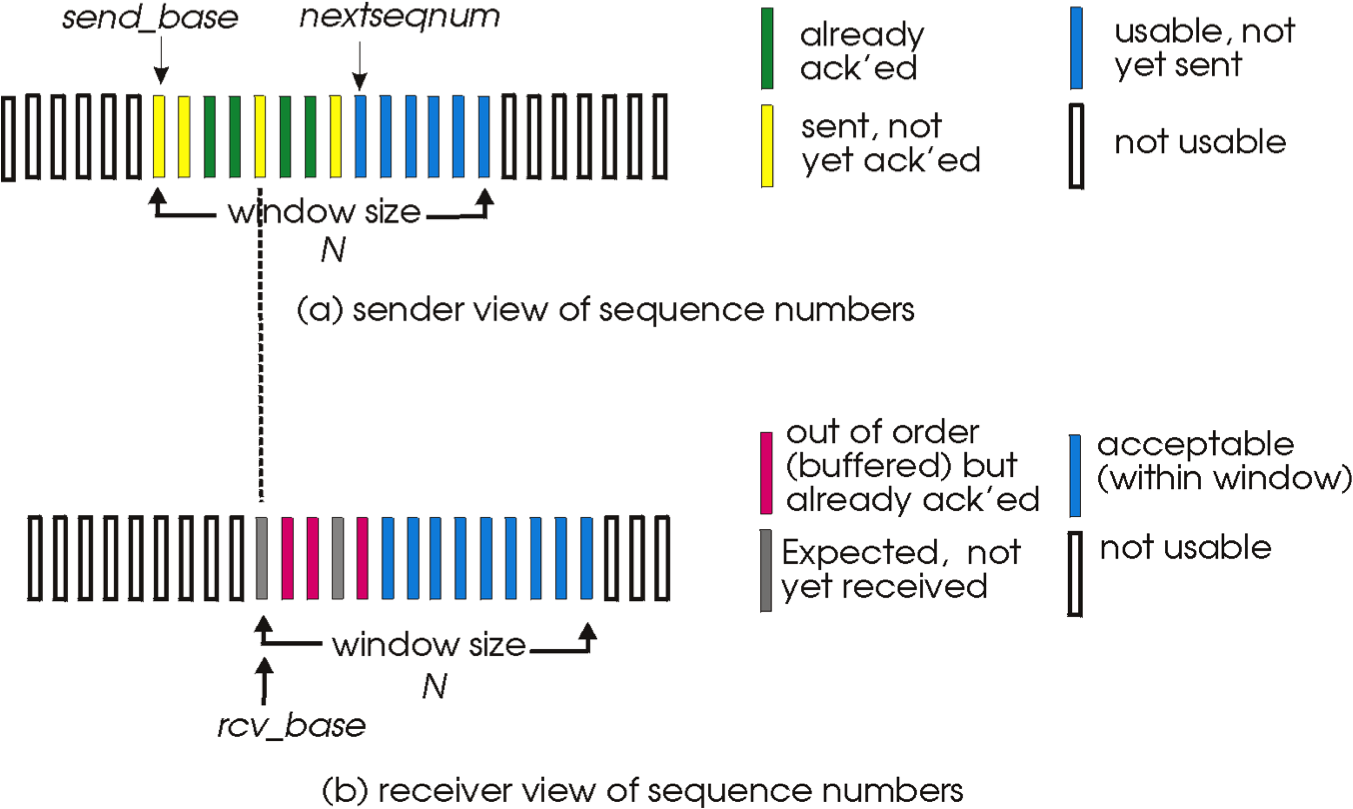
\includegraphics[width=11cm]{figs/08-rdt-13.png}
  \end{center}

\end{frame}
%---------------------------------------------------------------------
\begin{frame}
  \frametitle{{\em Reliable Data Transfer}}
  \framesubtitle{Repetición Selectiva}

  \begin{center}
    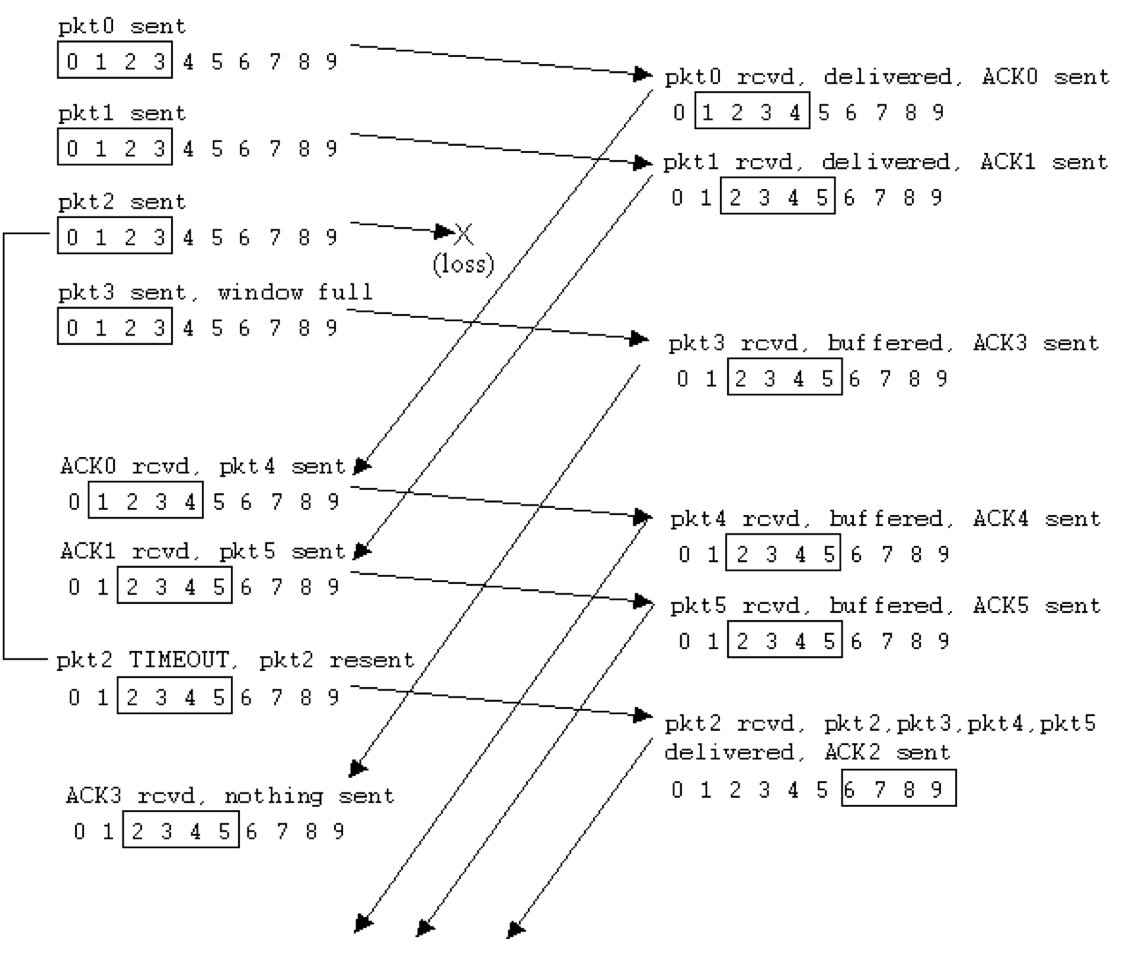
\includegraphics[width=8cm]{figs/08-rdt-14.png}
  \end{center}


\end{frame}

%---------------------------------------------------------------------
\begin{frame}
  \frametitle{Entonces ... ¿TCP?}
  \framesubtitle{Transmission Control Protocol}

  \begin{itemize}
    \item Protocolo de transmisión fiable
    \item Transmisión encadenanada ({\em chained})
      \begin{itemize}
        \item Gestiona control de flujo a través del tamaño de la ventana
      \end{itemize}
    \item Buffer en emisor y en receptor
    \item Orientado a conexión
      \begin{itemize}
        \item Protocolo de establecimiento de conexión antes de enviar paquetes de datos
      \end{itemize}
  \end{itemize}

\end{frame}

%---------------------------------------------------------------------
\begin{frame}
  \frametitle{TCP}
%  \framesubtitle{Transmission Control Protocol}

  Segmento TCP
  \begin{center}
    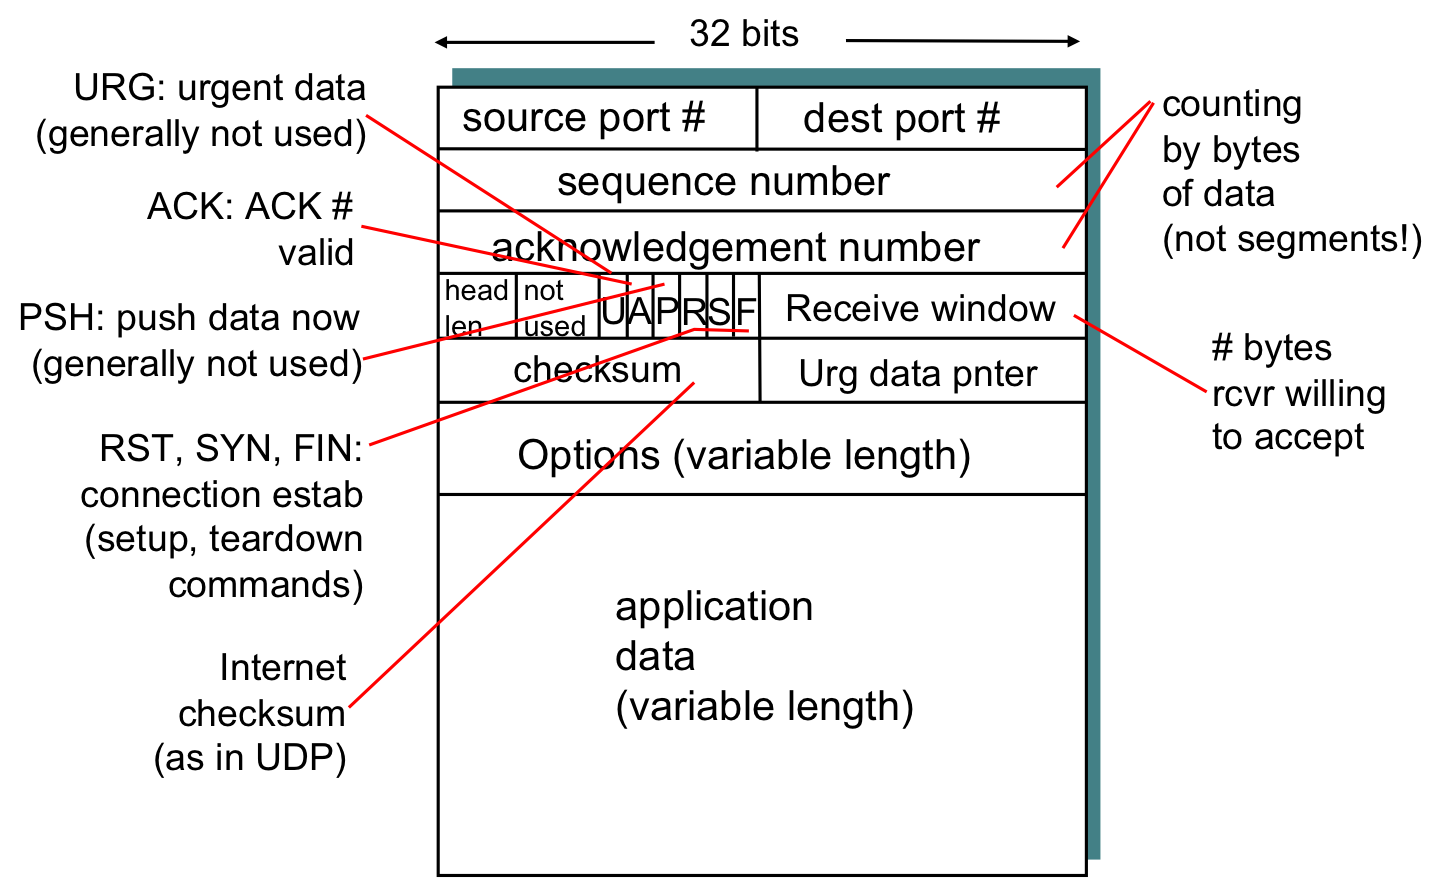
\includegraphics[width=10cm]{figs/08-tcp-header.png}
  \end{center}

\end{frame}
%---------------------------------------------------------------------
\begin{frame}
  \frametitle{TCP}

  Números de secuencia y ACKs
  \begin{center}
    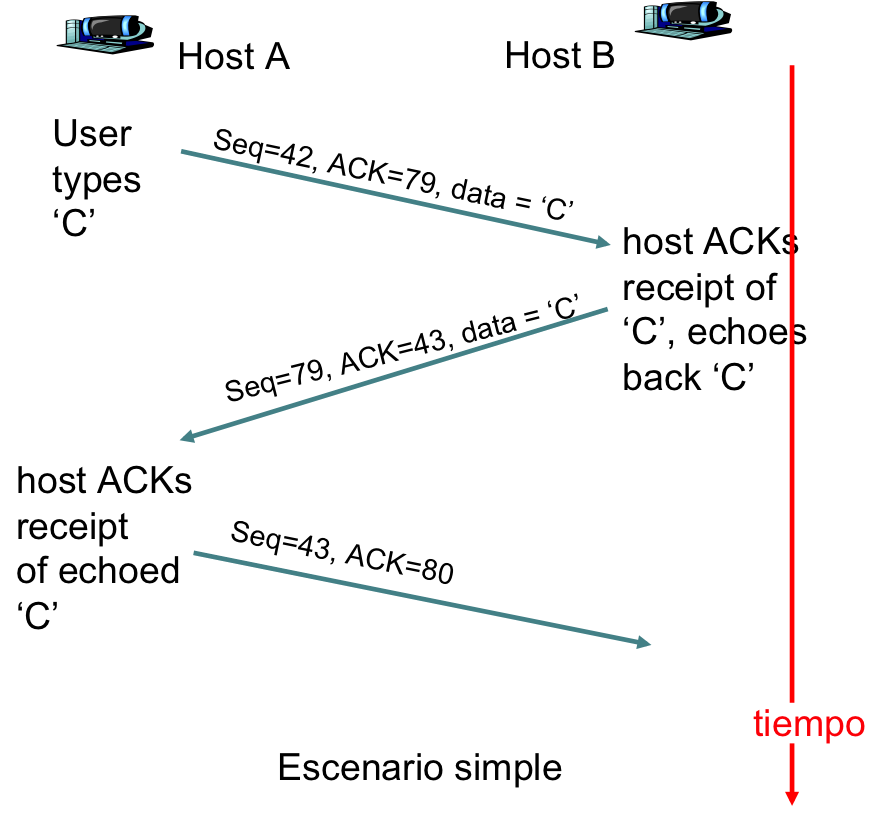
\includegraphics[width=6cm]{figs/08-tcp-seq.png}
  \end{center}

  ACKs puede ser agregados ({\em piggybacked}) en mensajes siguientes
\end{frame}
%---------------------------------------------------------------------
\begin{frame}
  \frametitle{TCP}

  Timeout TCP: ¿cómo estimarlo?
  \begin{itemize}
    \item Estimación muy corta: muchos timeout
    \item Estimación muy larga: reacción lenta a errores
  \end{itemize}
  Estimación de RTT
  \begin{itemize}
    \item Se mide repetidamente el RTT
    \item {\em SampleRTT}: tiempo desde envío hasta recepción de ACK
      \begin{itemize}
        \item Se mantiene promedio de últimos RTT
      \end{itemize}
    \item {\em EstimatedRTT}: se obtiene mediante media ponderada con decrecimiento exponencial
      \[ \text{EstimatedRTT} = (1-\alpha) \times \text{EstimatedRTT} + \alpha \times \text{SampleRTT} \]
  \end{itemize}
\end{frame}
%---------------------------------------------------------------------
\begin{frame}
  \frametitle{TCP}

  \begin{center}
    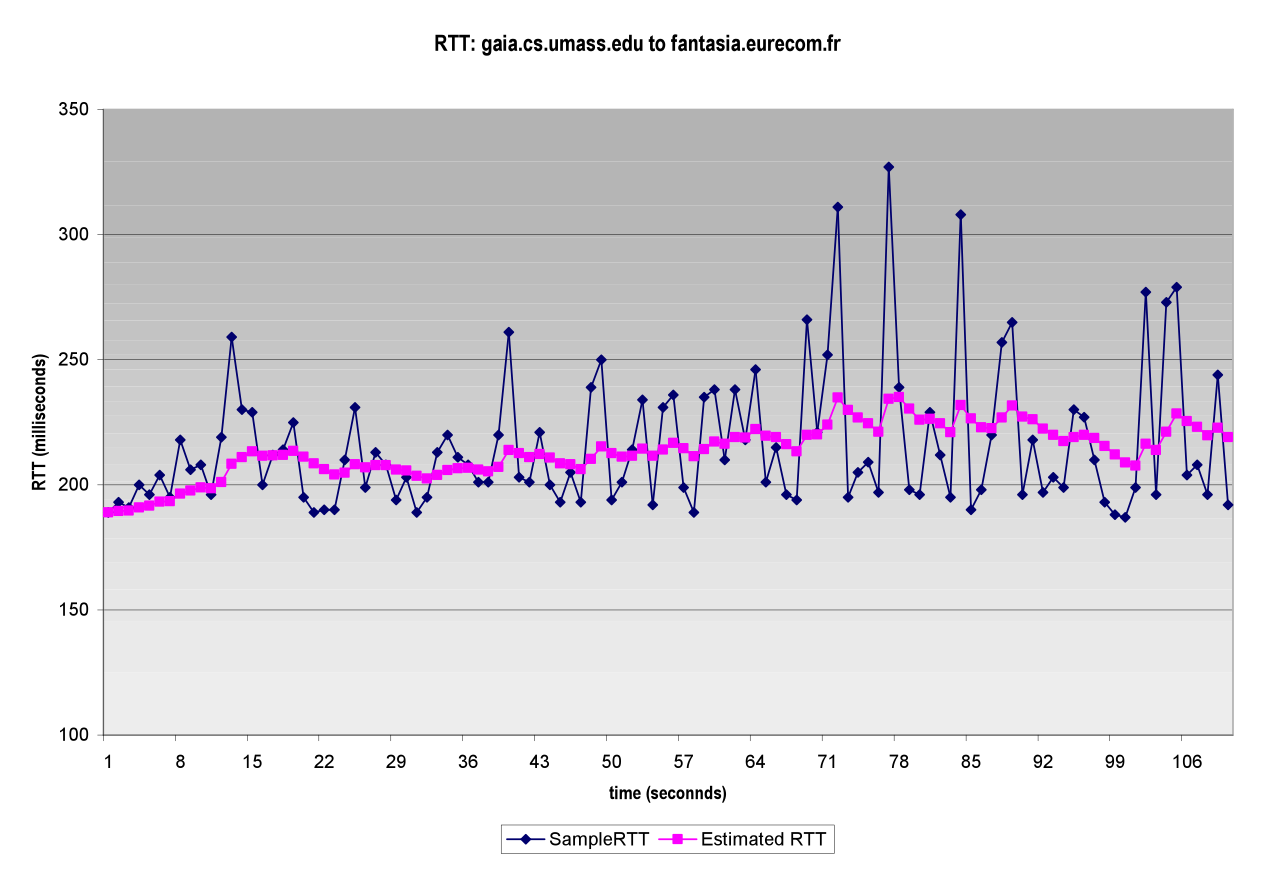
\includegraphics[width=11cm]{figs/08-tcp-estimation.png}
  \end{center}

\end{frame}


%---------------------------------------------------------------------
\begin{frame}
  \frametitle{TCP}
  \framesubtitle{Transferencia fiable}

  \begin{itemize}
    \item Segmentos encadenados
    \item ACKs acumulativos
    \item Timer de retransmisión único
  \end{itemize}
  Retransmite en:
  \begin{itemize}
    \item Timeout
    \item ACKs duplicados
  \end{itemize}


\end{frame}

%---------------------------------------------------------------------
\begin{frame}
  \frametitle{TCP}

  Algoritmo de transmisión fiable de TCP
  \begin{center}
    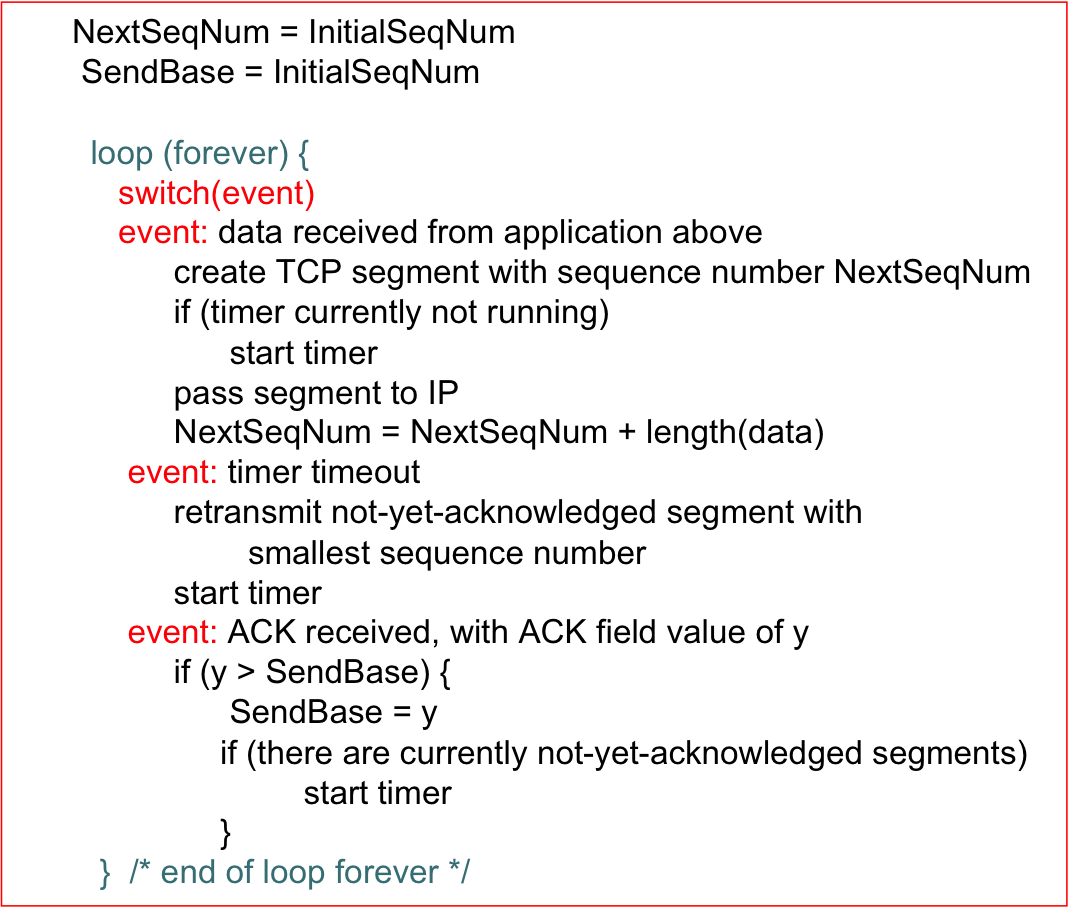
\includegraphics[width=8cm]{figs/08-tcp-send-algorithm.png}
  \end{center}

\end{frame}

%---------------------------------------------------------------------
\begin{frame}
  \frametitle{TCP}

  \begin{center}
    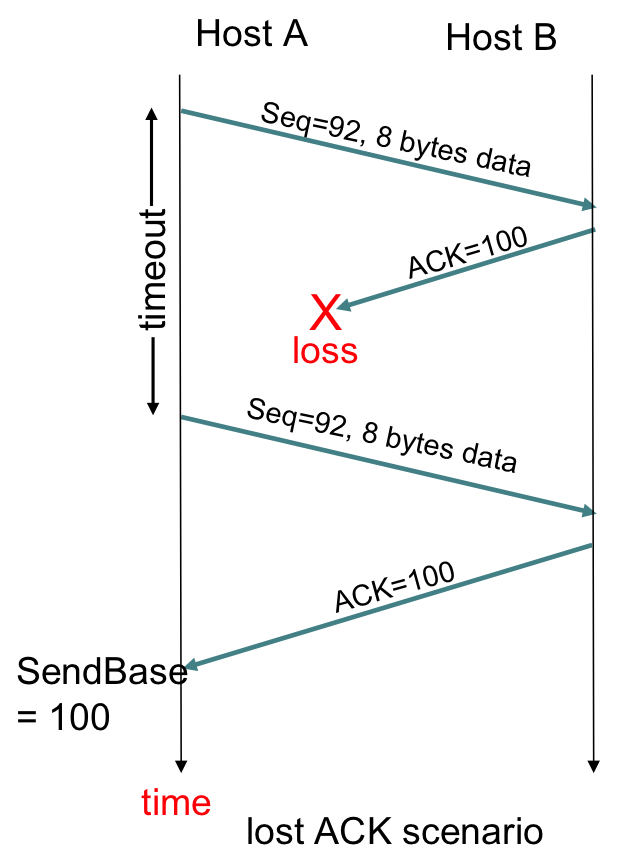
\includegraphics[width=5cm]{figs/08-tcp-reliable-1.png}
  \end{center}

\end{frame}


%---------------------------------------------------------------------
\begin{frame}
  \frametitle{TCP}

  \begin{center}
    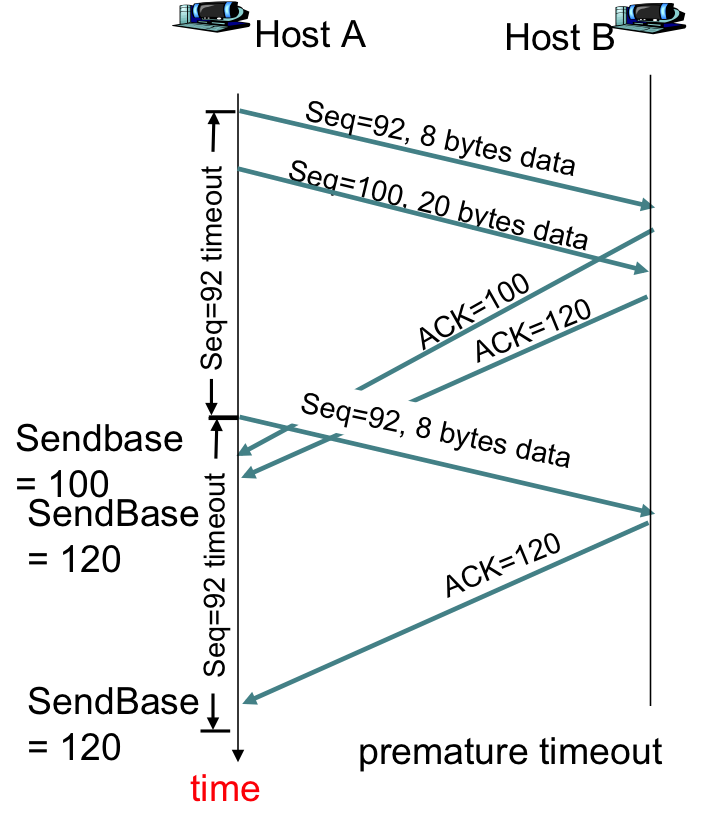
\includegraphics[width=6cm]{figs/08-tcp-reliable-2.png}
  \end{center}

\end{frame}


%---------------------------------------------------------------------
\begin{frame}
  \frametitle{TCP}

  \begin{center}
    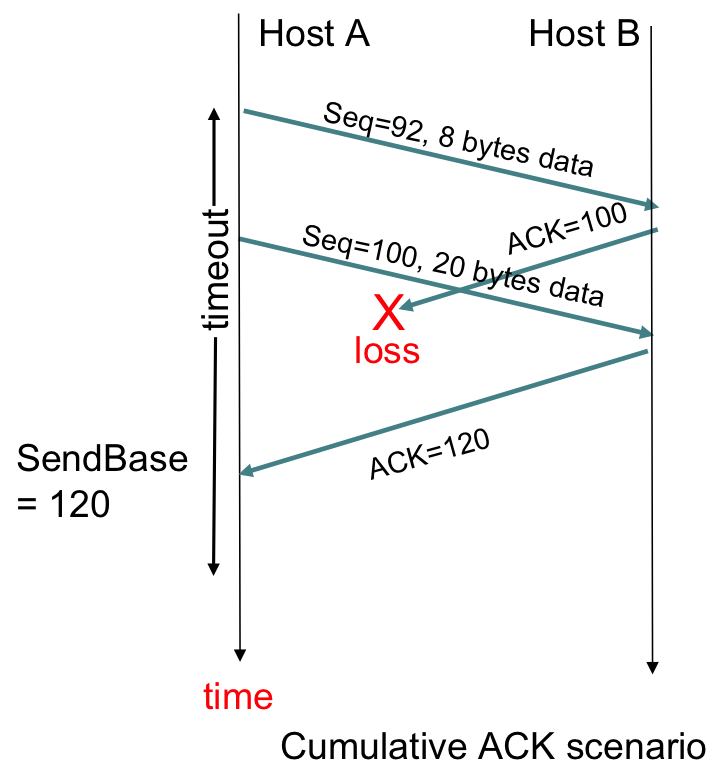
\includegraphics[width=6cm]{figs/08-tcp-reliable-3.png}
  \end{center}

\end{frame}

%---------------------------------------------------------------------
\begin{frame}
  \frametitle{TCP}
  Retransmisión rápida
  \begin{itemize}
    \item {\em Timeout}s pueden tomar mucho tiempo
    \item Retransmisión rápida envía proactivamente segmentos probablemente perdidos,
          antes de que ocurra un timeout
  \end{itemize}
  
  \begin{center}
    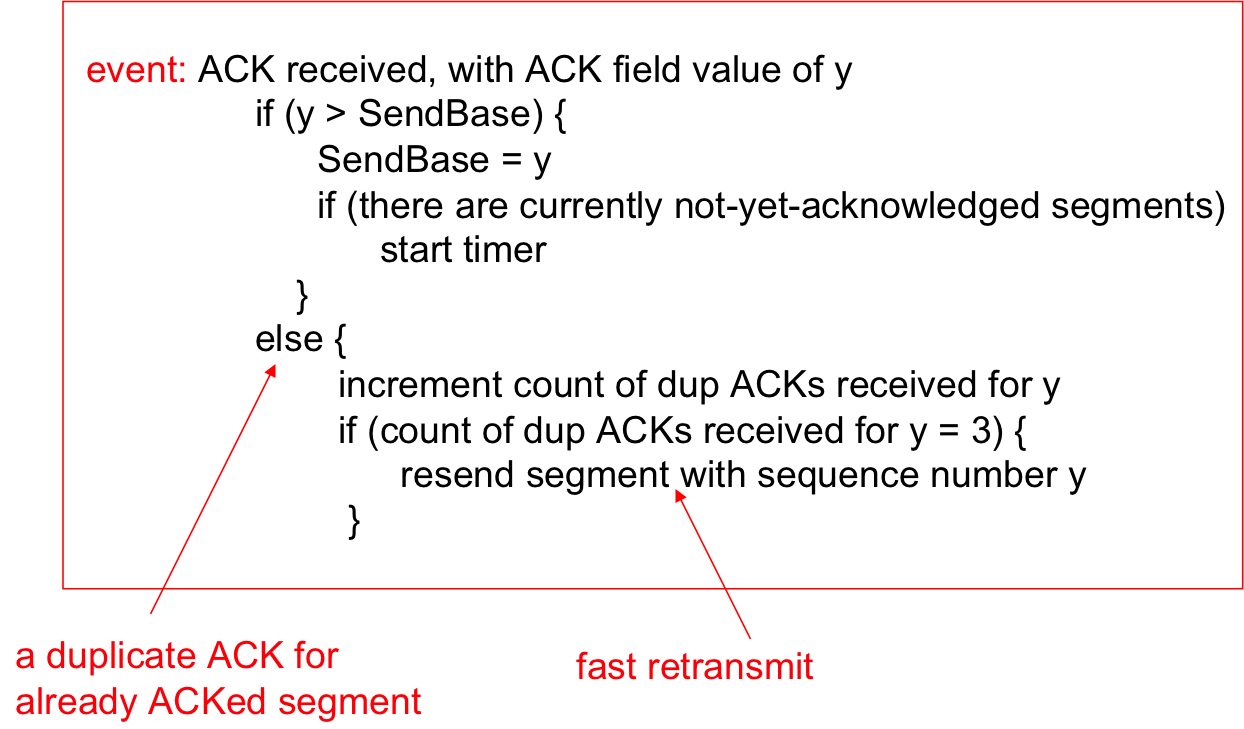
\includegraphics[width=8cm]{figs/08-tcp-retransmisionrapida.png}
  \end{center}

\end{frame}
  
%---------------------------------------------------------------------
\begin{frame}
  \frametitle{TCP}
  Retransmisión rápida

  \begin{center}
    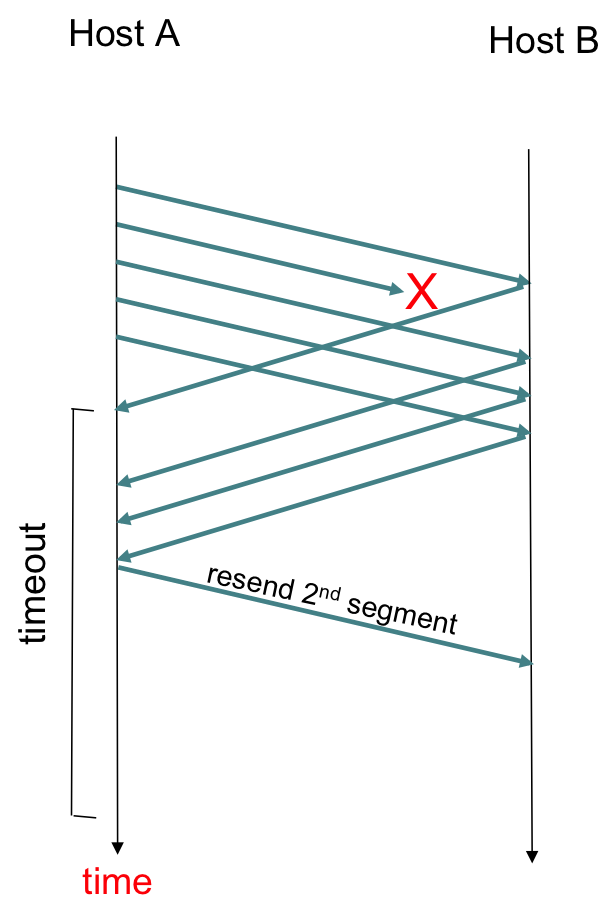
\includegraphics[width=4cm]{figs/08-tcp-retransmisionrapida-2.png}
  \end{center}


\end{frame}
%---------------------------------------------------------------------
\begin{frame}
  \frametitle{TCP}
  Control de Flujo
  
  \begin{center}
    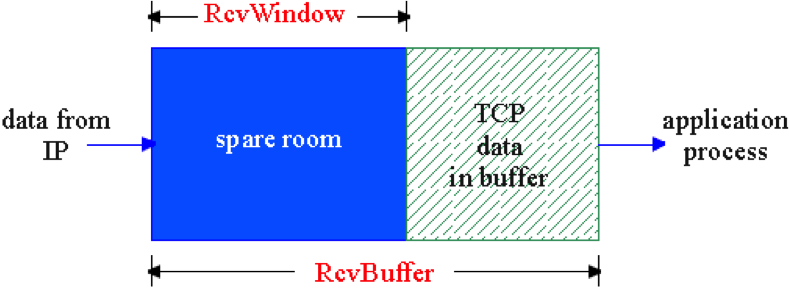
\includegraphics[width=6cm]{figs/08-tcp-flow.png}
  \end{center}
  
  \begin{itemize}
    \item Emisor no debe saturar al receptor
    \item Procesos en el receptor pueden demorarse en leer datos
    \item Receptor anuncia su espacio libren {\em buffer}: {\em RcvWindow}
    \item Emisor no envía más datos que los que quepan en {\em RcvWindow}
    \item Si no hay control de flujo (UDP), paquetes que no pueden ser recibidos se descartan
  \end{itemize}

\end{frame}
%---------------------------------------------------------------------
\begin{frame}
  \frametitle{TCP}
  \framesubtitle{Establecimiento de Conexión}
  TCP Handshake Protocol
  \begin{itemize}
    \item Paso 1. Cliente envía segmento {\tt SYN} al servidor
      \begin{itemize}
        \item Incluye número de secuencia inicial
      \end{itemize}
    \item Paso 2. Servidor recibe {\tt SYN}, y responde con {\tt SYN ACK}
      \begin{itemize}
        \item Servidor asigna buffer
        \item Servidor establece número de secuencia inicial
      \end{itemize}
    \item Paso 3. Cliente recibe {\tt SYN ACK}, y responde con {\tt ACK}
      \begin{itemize}
        \item Este paquete ya puede contener datos
      \end{itemize}
  \end{itemize}

\end{frame}
%---------------------------------------------------------------------
\begin{frame}
  \frametitle{TCP}
  \framesubtitle{Establecimiento de Conexión}
  TCP Cierre de Conexión
  \begin{itemize}
    \item Paso 1. Cliente envía {\tt FIN} al servidor
    \item Paso 2. Servidor recibe FIN, responde con {\tt ACK}, cierra conexión y envía {\tt FIN}
    \item Paso 3. Cliente recibe {\tt FIN}, responde con {\tt ACK}, cerrará conexión después de timeout.
    \item Paso 4. Servidor recibe ACK, cierra conexión.
  \end{itemize}

\end{frame}
%---------------------------------------------------------------------
\begin{frame}
  \frametitle{TCP}
  \framesubtitle{Establecimiento de Conexión}

  \begin{center}
    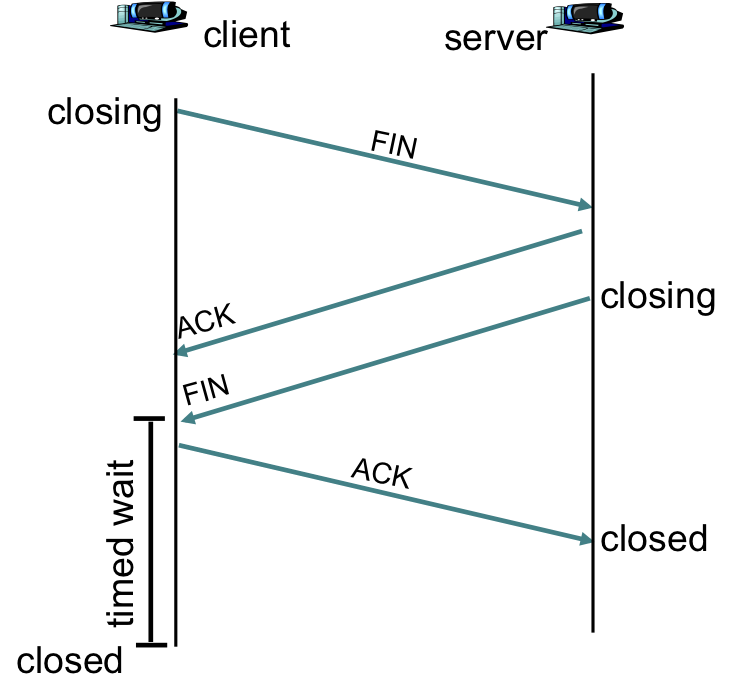
\includegraphics[width=6cm]{figs/08-tcp-close.png}
  \end{center}


\end{frame}

%---------------------------------------------------------------------
\begin{frame}
  \frametitle{TCP}
  \framesubtitle{Ciclo de vida de Cliente TCP}

  \begin{center}
    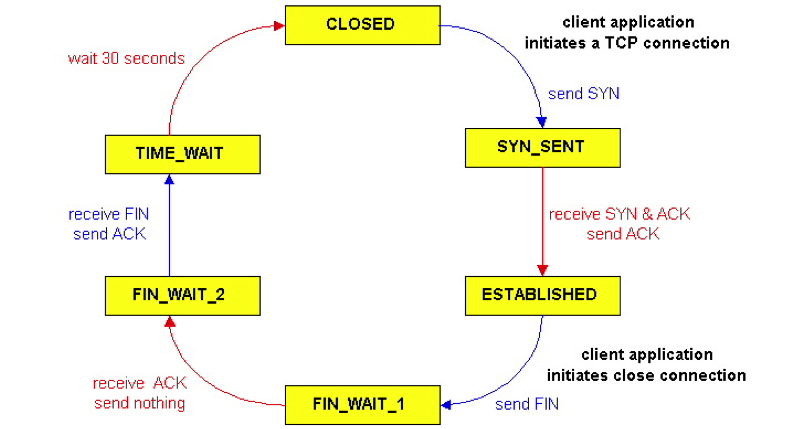
\includegraphics[width=10cm]{figs/08-tcp-client-lc.png}
  \end{center}

\end{frame}
%---------------------------------------------------------------------
\begin{frame}
  \frametitle{TCP}
  \framesubtitle{Ciclo de vida de Servidor TCP}

  \begin{center}
    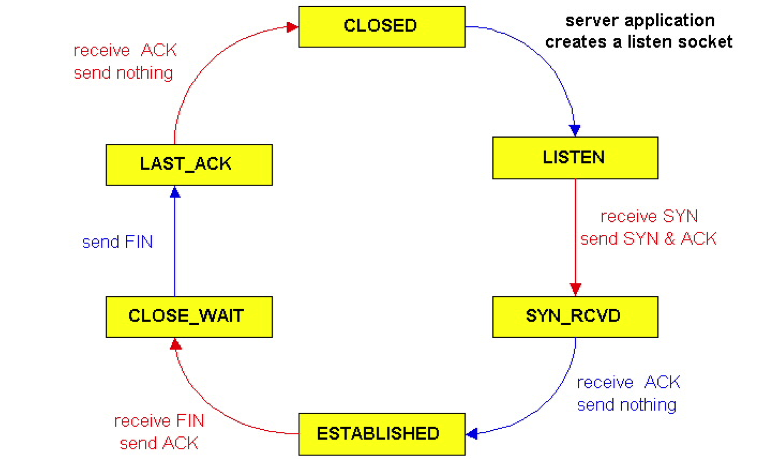
\includegraphics[width=10cm]{figs/08-tcp-server-lc.png}
  \end{center}

\end{frame}
%---------------------------------------------------------------------
\end{document}